\documentclass[10pt,a4paper,twoside,twocolumn]{article}%ustalasz jaki typ dokumentu i właściwości

\usepackage[polish]{babel} % ustawianie języka polskiego
\usepackage[colorlinks=false,linkcolor=green,urlcolor=green,citecolor=green]{hyperref}%hiperłącza ogólnego rodzaju
\hypersetup{pdftitle=Sprawozdanie SSR}

\usepackage{pdfpages} % importowanie plików z pdfa
\usepackage{amsmath} % do wstawiania macierz itp
\usepackage{graphicx} % wstawianie zdjęć
% \usepackage[utf8]{inputenc} % niepotrzebne bo lualatex
\usepackage[T1]{fontenc} % niepotrzebne bo lualatex
\usepackage[left=1cm,right=1cm,top=1cm,bottom=2cm,
columnsep=1cm % odstęp między kolumnami
]{geometry}%marginesy

\usepackage{listings} % punktowanie
% \usepackage{indentfirst} % dawanie akapitu na początku
\usepackage{caption} % podpisy
\usepackage{siunitx} % jednostki si
\usepackage{minted} % ładne kody naprzyklad matlaba
\setminted{linenos=true,frame=single,breaklines=true,breaksymbolleft=}

\usepackage{textcase}

\usepackage[polish,nameinlink]{cleveref} % dobre prefiksy przed etykietą i język
\usepackage{cprotect}

\usepackage{fontspec}
% \setmainfont[Ligatures=TeX]{Georgia}
% \setsansfont[Ligatures=TeX]{Arial}
\usepackage{parskip} % usunięcie tab na początku akapitu
\usepackage{float} % aby można było ładnie wstawić elementy typu zdjecie, kod itp

%%% rysowanie wykresów %%% ale w ciul to trudne więc app.diagrams.net
\usepackage{tikz}
\usetikzlibrary{shapes.geometric, arrows, positioning}

% % % SVG import
\usepackage{svg}
\usepackage{import}
\usepackage{xifthen}
\usepackage{transparent}


%%%%%%%%%%%%%% koniec pakietów %%%%%%%%%%%%%%%%%%%%%%%%%%%



\title{Fajny ten tytuł}%tytuł
\date{\today}%%data
\author{Janusz Chmaruk}%autor
\setcounter{secnumdepth}{3}%głębokość liczenia roździałów


%%%%%%%%%%%%%%%%%%%%%%%%%%%%%%%%%%%%%%%%%%%%%%%%%%%%%%%%%%%%%%%
%%%%%%%%%%%%%%%%%%%%%%%%%%%%%%%%%%%%%%%%%%%%%%%%%%%%%%%%%%%%%%%
%%%%%%% TU SIE ZACZYNA PISANIE PLIKU %%%%%%%%%%%%%%%%%%%%%%%%%%
%%%%%%%%%%%%%%%%%%%%%%%%%%%%%%%%%%%%%%%%%%%%%%%%%%%%%%%%%%%%%%%
%%%%%%%%%%%%%%%%%%%%%%%%%%%%%%%%%%%%%%%%%%%%%%%%%%%%%%%%%%%%%%%

\begin{document}%zaczyna się dokument

\null%

\includepdf[pages={1}]{Szablon_Projektu.pdf}
\clearpage%następna strona ogółem

\tableofcontents%spis treści
% \clearpage

\section{Wstęp}
Celem ćwiczenia jest zapoznanie z tworzeniem własnych formatów wiadomości w
systemie ROS.
\section{Zakres ćwiczenia}
\begin{itemize}
    \item Tworzenie własnych formatów wiadomości
    \item Obsługa czasu w systemie ROS
    \item Tworzenie wykresów przy pomocy narzędzia rqt\_plot
\end{itemize}
\section{Realizacja ćwiczenia}
\subsection{Tworzenie własnego typu wiadomości}
\textit{W nowej paczce utwórz własny typ wiadomości Student o następujących
polach: numer\_albumu, imię, nazwisko, aktywny, oceny, kierunek. Napisz w
dowolnym języku program nasłuchujący wiadomości na topicu /student i wypisujący
ich zawartość do logu.}


W podanym tekście opisano proces tworzenia, wysyłania i odbierania własnej
wiadomości w systemie ROS (Robot Operating System). Omówiono elementy kodu
publishera i subscribera oraz przedstawiono wyniki ich działania na zrzucie
ekranu z terminala. Rys.1 przedstawia format utworzonej wiadomości. Kod
publishera, który wysyła wiadomość o utworzonym formacie, pokazano na Rys.2.
Wiadomość jest wysyłana na temacie /student z kolejką wynoszącą 10 wiadomości. W
kodzie publishera linijka 6 uruchamia węzeł o nazwie student, a linijka 7
definiuje temat, format wiadomości i wielkość kolejki dla publishera. W linii
10-16 przypisywane są dane do poszczególnych składowych wiadomości, a ostatnia
komenda wysyła utworzoną wiadomość. Kod subscribera, który nasłuchuje na temacie
/student, znajduje się na Rys.3. W linii 6 kodu subscribera (Rys. 3) utworzono
funkcję odbierającą wiadomość z tematu /student o nowym formacie i wyświetlającą
odebrane dane. W linii 9 uruchamiany jest węzeł o nazwie student\_listener, a w
linii 11 zdefiniowano funkcję subscribera, określając temat do nasłuchiwania,
oczekiwany typ wiadomości i funkcję do wykonania po otrzymaniu wiadomości.
Funkcja rospy.spin() odpowiada za aktualizację zdarzeń systemu ROS. Na Rys. 4
przedstawiono zrzut ekranu z terminala, na którym widać działanie publishera
wysyłającego dane oraz subscribera odbierającego wiadomość.


\begin{figure}[H]
    \centering
    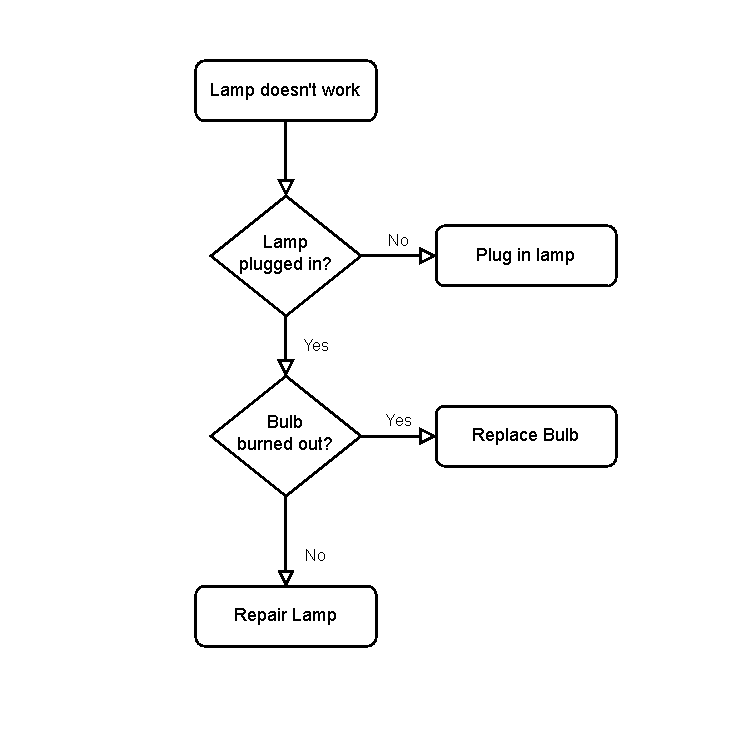
\includegraphics[width=1\linewidth]{1234.pdf}
    \caption{heading}
\end{figure}


\begin{figure}[H]
    \centering
    \begin{verbatim}
        uint32 numer_albumu
        string imie
        bool aktywny
        float32[] oceny
        string kierunek
    \end{verbatim}
    \caption{Utworzony typ wiadomości w pliku Student.msg}
\end{figure}


%
\begin{figure}[H]
    \centering
    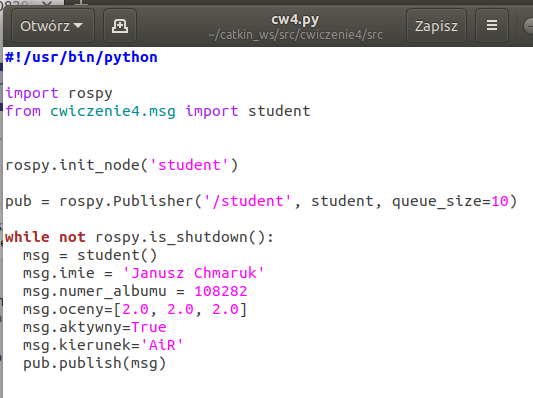
\includegraphics[width=0.8\linewidth]{cw4_py.png}
    \caption{Kod publishera wykonany w języku python}
\end{figure}

\begin{figure}[H]
    \centering
    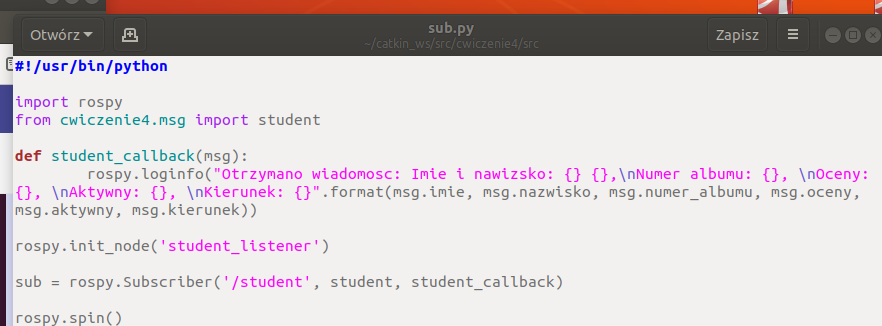
\includegraphics[width=1\linewidth]{sub_py.png}
    \caption{Kod subscribera wykonany w języku python}
\end{figure}

\begin{figure}[H]
    \centering
    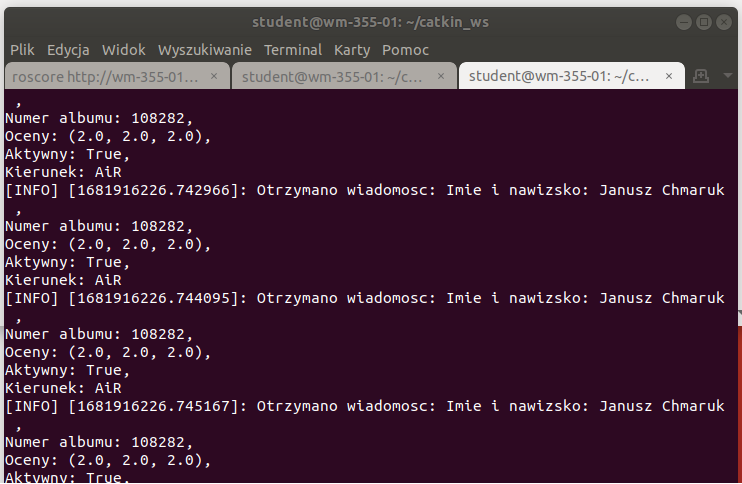
\includegraphics[width=1\linewidth]{konsola.png}
    \caption{Efekt działania utworzonego publishera oraz subscribera}
\end{figure}

\subsection{Węzeł alarmujący}
\textit{Napisz program, który będzie alarmował o przekroczeniu dozwolonego stanu
parametru procesu (np. temperatura w piecu). Program powinien nasłuchiwać na
pewnym topicu aktualnej wartości stanu procesu, a w przypadku przekroczenia jej
górnego lub dolnego limitu wysyłać wiadomość zawierającą: stan alarmu, który
limit został przekroczony, o ile limit został przekroczony, oraz jak długo trwa
stan alarmu. Sprawdź działanie programu. Wykreśl przy pomocy programu rqt\_plot
wykres obserwowanej wartości i określ, czy alarmy zostały poprawnie zgłoszone.}

\begin{figure}[H]
    \centering
    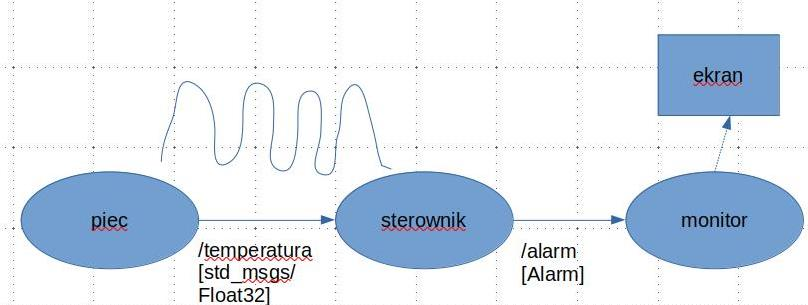
\includegraphics[width=\linewidth]{1.png}
    \caption{Schemat układu do zadania 2}
\end{figure}

W drugim zadaniu stworzono dwa nowe typy wiadomości: regulacja (Rys\@. 6) oraz
alarm (Rys\@.7). Aby zwiększyć czytelność sygnałów alarmowych w narzędziu
rqt\_plot, alarmy utworzono jako typ int32, przyjmujący wartość równą dozwolonym
zakresom. Te wartości to 1500 dla tempmax i 700 dla tempmin. Na Rys\@. 8
przedstawiono kod programu piec.py, który tworzy sygnał sinusoidalny i przesyła
go na temacie /temperatura. Kod programu sterownik.py, który nasłuchuje
wiadomości na temacie /temperatura i sprawdza, czy przekroczone zostały
dopuszczalne zakresy temperatur pieca, pokazano na Rys\@. 9. Następnie sterownik.
py wysyła informacje o alarmach na temacie /alarm. Rys\@. 10 zawiera kod programu
ekran.py, który odbiera i wyświetla informacje z tematów /temperatura oraz
/alarm. Gdy wystąpi stan alarmowy, ekran.py oblicza czas trwania alarmu oraz
wartość, o jaką został przekroczony zakres. Zrzut ekranu z terminala w trakcie
działania tych programów można zobaczyć na Rys\@. 11.

\begin{figure}[H]
    \centering
    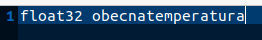
\includegraphics[width=0.6\linewidth]{2.png}
    \caption{Utworzony typ wiadomości temperatura}
\end{figure}

\begin{figure}[H]
    \centering
    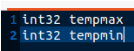
\includegraphics[width=0.4\linewidth]{3.png}
    \caption{Utworzony typ wiadomości alarm}
\end{figure}

\begin{figure}[H]
    \centering
    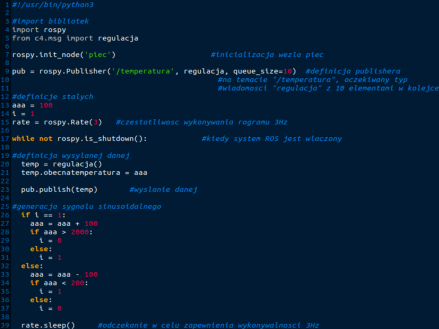
\includegraphics[width=\linewidth]{4.png}
    \caption{Utworzony program piec.py, w którym został umieszczony
    publisher wysyłający wiadomość temperatura na temacie /temperatura}
\end{figure}

\begin{figure}[H]
    \centering
    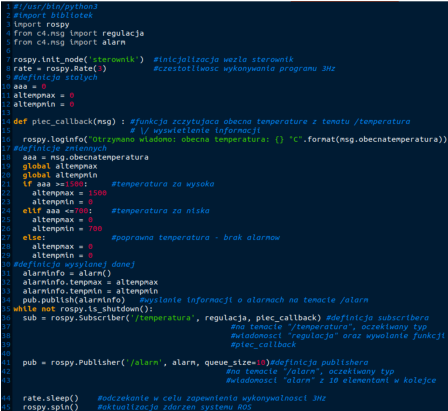
\includegraphics[width=\linewidth]{5.png}
    \caption{Utworzony program sterownik\@.py zawierający subscribera
    odbierającego wiadomości na temacie /temperatura oraz publishera
    wysyłającego wiadomość typu alarm na temacie /alarm}
\end{figure}

\begin{figure}[H]
    \centering
    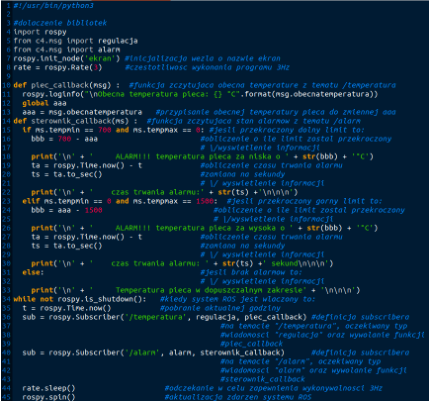
\includegraphics[width=\linewidth]{6.png}
    \caption{Utworzony program ekran\@.py, który posiada dwa subscribery
    nasłuchującego wiadomości na temacie /temperatura oraz /alarm}
\end{figure}

\begin{figure}[H]
    \centering
    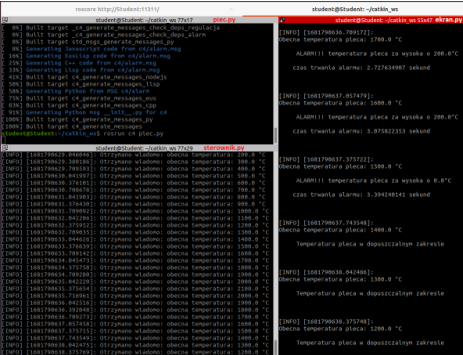
\includegraphics[width=\linewidth]{7.png}
    \caption{Efekt działania utworzonych programów piec\@.py, sterownik\@.py
    oraz ekran\@.py}
\end{figure}

Po przetestowaniu działania programu, przy pomocny węzła rqt\_plot zostały
wyznaczone przebiegi czasowe zawierające temperaturę pieca oraz sygnały alarmowe
\begin{itemize}
    \item tempmax - informujący o przekroczeniu górnego zakresu temperatury,
    \item tempmin - informujący o przekroczeniu dolnego zakresu temperatury.
\end{itemize}


\begin{figure}[H]
    \centering
    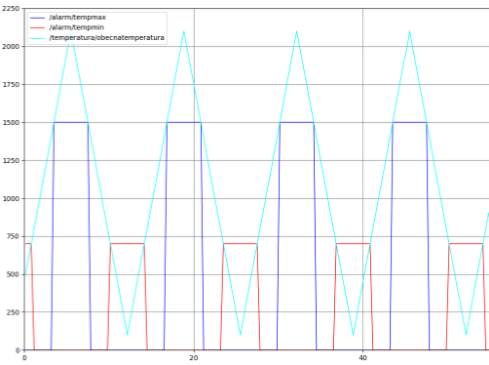
\includegraphics[width=\linewidth]{8.png}
    \caption{Zarejestrowane przebiegi sygnałów z wykorzystaniem narzędzia rqt\_plot}
\end{figure}

Program działa zgodnie z początkowymi założeniami. Zarejestrowane przebiegi są
prawidłowe tzn. alarmy pojawiają się oraz znikają w chwilach wyjścia/wejścia z
zakresu wielkości procesowej (temperatury).

\section{Wnioski}
Realizacja ćwiczenia pozwoliła na zapoznanie się z procesem tworzenia własnych
typów wiadomości w systemie ROS. Ważne jest, aby pamiętać o modyfikacji plików
cmakelist.txt oraz package.xml, które znajdują się w katalogu tworzonej paczki w
przestrzeni roboczej, np. \textasciitilde /catkin\_ws/src/c4. Narzędzie
rqt\_plot umożliwia śledzenie przebiegów wybranych zmiennych. Przy korzystaniu z
tego narzędzia warto ustawić odpowiednie zakresy osi X i Y, gdyż domyślne
wartości mogą być niewystarczające. Podczas pracy z systemem ROS niezbędne jest
uruchomienie węzła centralnego za pomocą polecenia roscore. Nieuruchomienie lub
wyłączenie węzła centralnego uniemożliwi nawiązanie połączenia pomiędzy nowo
otwartymi programami. Warto jednak zauważyć, że wyłączenie węzła centralnego nie
wpływa na działanie węzłów, które już komunikują się ze sobą.

\end{document}